\documentclass[]{article}
%opening
\title{Writeup Document}
\author{Alex Miller}
\addtolength{\oddsidemargin}{-.875in}
\addtolength{\evensidemargin}{-.875in}
\addtolength{\textwidth}{1.75in}
\addtolength{\topmargin}{-.875in}
\addtolength{\textheight}{1.75in}
\setcounter{secnumdepth}{0}
\usepackage{cancel}
\usepackage{amssymb}
\usepackage{amsmath}
\usepackage{hyperref}
\usepackage{graphicx}
\graphicspath{ {./} }
\usepackage[ruled,vlined, linesnumbered]{algorithm2e}
\DontPrintSemicolon


\begin{document}
\maketitle

\section{Changes}
\subsection{Changes to the design}
The following addresses changes I have made to my projects design, broken down by module:
\begin{itemize}
	\item Top level modules (serial.c, parallel.c, my\_test\_serial.c, my\_test\_parallel.c) -- These files will take in the same inputs and utilize the same basic functionality as previously described in my design document. The following aspects will be modified
	
	\textbf{serial.c and parallel.c}
	\begin{itemize}
		\item I originally proposed to perform the lock tests required by the assignment by comparing the runtimes for a serial counter as opposed to a parallel counter using my lock implementations. In order to implement comparable behavior between my serial and parallel counters, I thought that the serial counter should increment an integer within a single for-loop B times, while the parallel counter should launch N threads which each increment a shared counter B / N times.
		\\\\
		This Design went under two key revisions. The first was that the parallel counter was redesigned such that each thread, within an infinite while loop, acquires the lock, and checks whether a shared counter is less than B; if so, the given thread increments the shared counter, unlocks, and goes to the top of the while loop. Otherwise the thread unlocks and returns. 
		The parallel counter now also returns a long, instead of an int type.
		The motivation for this change was so that the critical section of the parallel counters would look more like that of the for loop described in the serial counter. Like a for loop, it involves checking whether an integer is less than B, and, if so, incrementing that integer. Otherwise each thread would have to maintain a shared counter which they would have to read and write each cycle, on top of incrementing the counter.
		\\\\
		The second change was to the serial counter. Like the parallel counter, it now returns a long. It initially was designed to check and increment a integer without the volatile attribute. However, when this approach was tested, the serial counter was able to output near-0 run times. This was probably due to compiler optimization. To mitigate this, as well as make the serial counter more like the parallel counter, the integer the serial counter uses has the volatile type, which stops the compiler from being able to make complicating optimizations.
	\end{itemize}
	\textbf{my\_test\_serial.c and my\_test\_parallel.c}
	\begin{itemize}
		\item $usleep()$ actually sleeps programs in microseconds, so instead, both my serial and parallel sleepers make their threads sleep for $usleep(t * 1000)$ microseconds at a time.
		
		Additionally, I also modified the functionality of the parallel sleeper in much the same way as I modified the parallel counter. Rather than each of the N threads sleeping for $usleep(t * 1000)$ microseconds $B / (t * n)$ times, each thread, within an infinite while loop, acquires the lock, and checks whether a shared counter is less than B; if so, the given thread increments the shared counter by t,  $usleep(t * 1000)$ microseconds, unlocks, and goes to the top of the while loop. Otherwise the thread unlocks and returns.
		This behavior mimics that of the serial sleeper, which has to utilize a for loop, without necessitating the use of extra confounding variables. The serial sleeper utilizes a volatile long to monitor progress in order to equalize performance even further.
	\end{itemize}
	\item Algorithm implementation level
	\\\\
	\textbf{lock.c}
	\begin{itemize}
		\item  I more thoroughly defined as well as changed the structure of my locking interface. I ended up defining my $lock\_methods$ struct under the struct name $lock_t$. The struct has the following attributes:
		\begin{itemize}
			\item char type : a reference to a lock type, as specified by input
			
			\item int B : The number threads should count/sleep to. I included this integer in order to make passing arguments to the threads as easy as passing them a pointer to this struct.
			
			
			\item int t : This integer is used in the sleeper function. 
			
			\item volatile long counter : The counter the threads share and increment.
			
			\item void *l : a pointer to a lock object; this pointer is passed to the initialization, lock, and unlock functions.
			
			\item void (*init\_thread)(void *) : This function initializes any thread specific structures required by a lock. It should be called before a thread acquires the lock the first time.
			
			\item void (*lock)(void *) : a pointer to the lock's lock function; it should be called on the void *l (which points to the initialized lock) in order to acquire the lock. 
			
			\item void (*unlock)(void *) : a pointer to the lock's unlock function; it should be called on the void *l (which points to the initialized lock) in order to release the lock. 
		\end{itemize}
		\item I defined an $init_thread$ function for each lock; this method simply returns for all locks except the MCS lock, which requires thread specific QNode structs, as defined in the textbook.
	\end{itemize}
	\item Testing script (test\_script.sh)
	\begin{itemize}
		\item Now that threads don't increment a shared counter an equal number of times, but instead perform an undetermined amount with the use of value checking, the $B$ values used in these tests no longer have to be multiples of $N$. Furthermore, $B = 1120$ did not seem sufficiently large enough to mitigate the effects of variation. Therefore, for all counter tests $B = 10000$ instead.
	\end{itemize}
\end{itemize}

\subsection{Changes to Test plan:}
I have not made any changes to my test plan. I want only to remark here that by only inferring the correctness of my locks through the output of the shared counter, we can only infer that all of our locks satisfy mutual exclusions. This does not prove that our FCS lock implementations preserve FCS ordering. However, as that would require time developing an additional testing structure, I am choosing not to implement that here.

\section{Results}
The raw performance data for the Idle Lock Overhead, Lock Scaling, and Proprietary tests are stored in a folder called $HW3a/hw3a/exp\_data$. This folder contains the .csv files that describe performance data for a given experiment. This data was collected by running implementations for given number of trials, calculating measurements per trial, and taking median values. As such there is no other collected data other than median speedup, worker rates, and dispatcher rates. That data was deleted as it did not serve the purpose of analysis and would've have complicated my data storage scheme.
\\\\
As per how many trials I utilized; for experiments utilizing uniform and constant packets, I used 5 trials. I though this was sufficient for our counter tests, and would have to suffice for my sleeper tests, as those take quite while (at least 3 seconds each).
\\\\
I took this data and plotted it using the script analyze.py. These graphs are stored in the folder $HW3a/Docs/graphs$. I will display these graphs below:

\subsection{Experiment 1: Idle Lock Overhead}
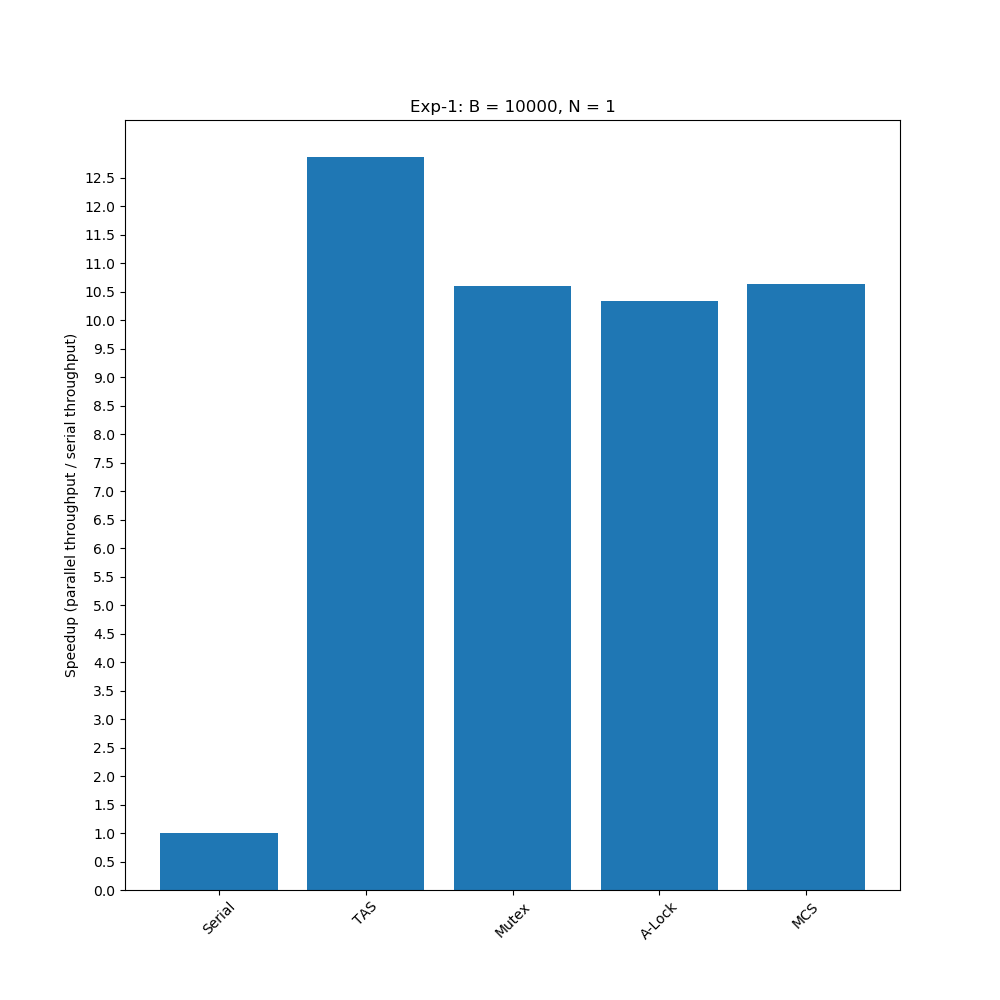
\includegraphics[scale=0.5]{graphs/exp1.png}\\
\subsection{Experiment 2: Lock Scaling}
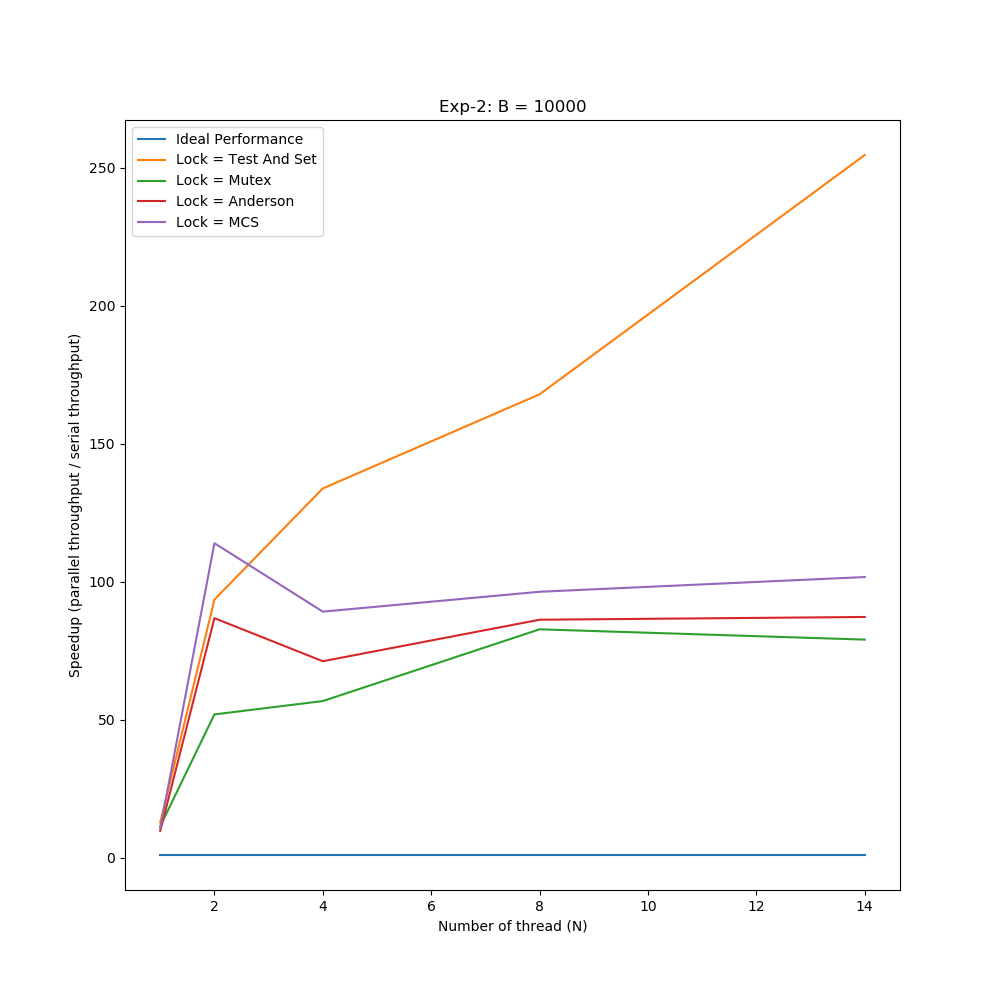
\includegraphics[scale=0.5]{graphs/exp2.png}\\
\subsection{Experiment 3: My Test}
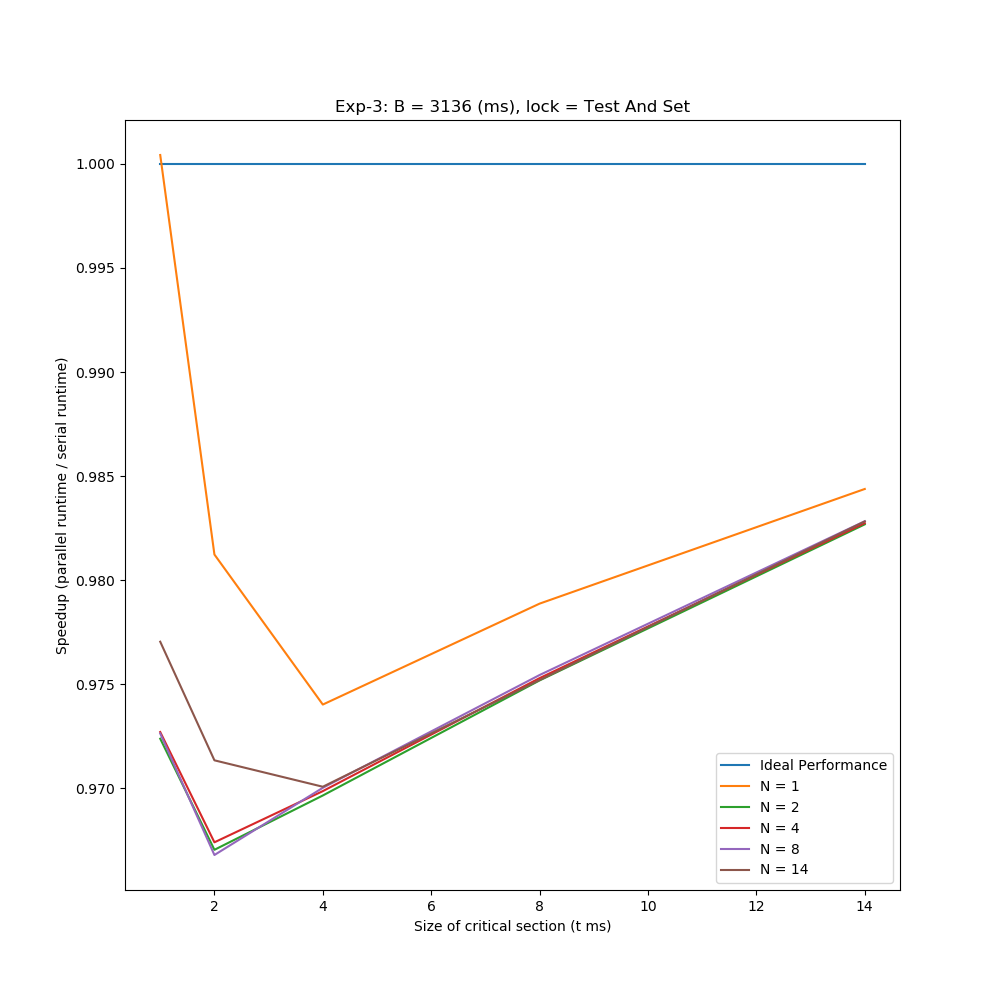
\includegraphics[scale=0.5]{graphs/exp3_t.png}\\
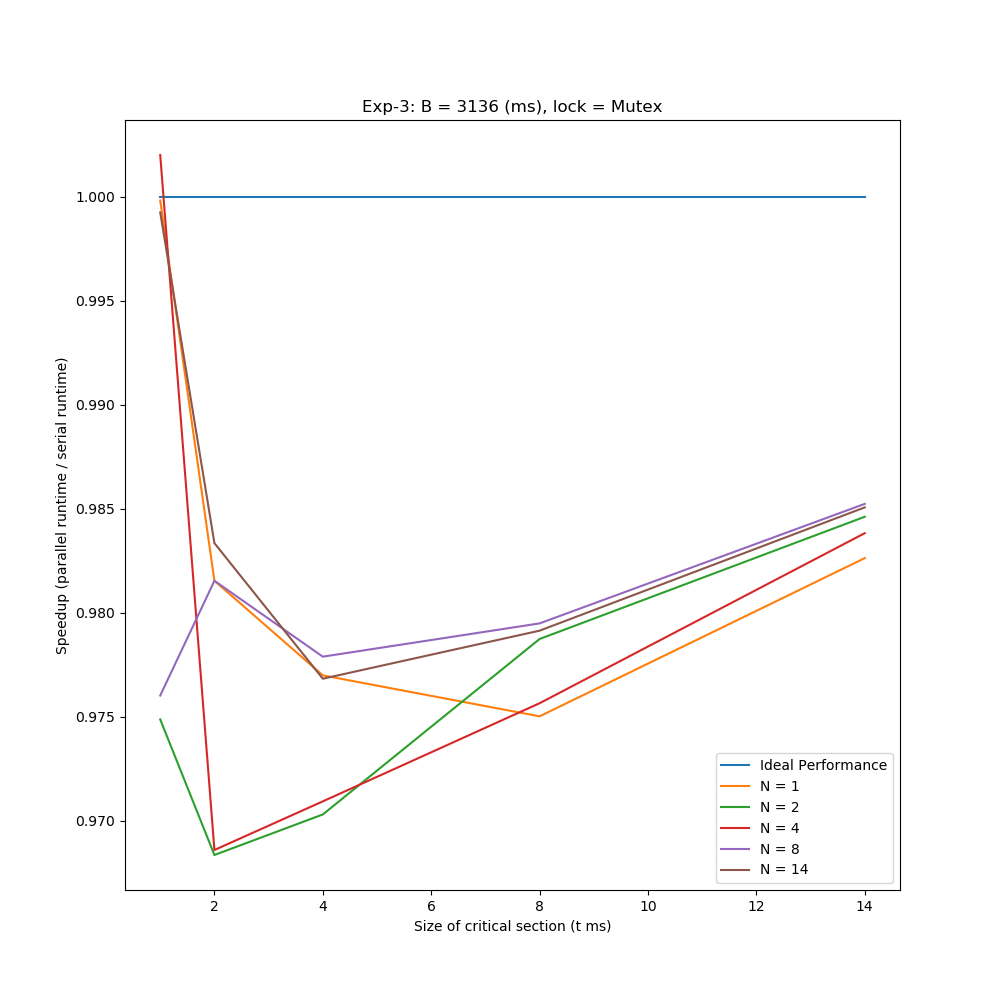
\includegraphics[scale=0.5]{graphs/exp3_p.png}\\
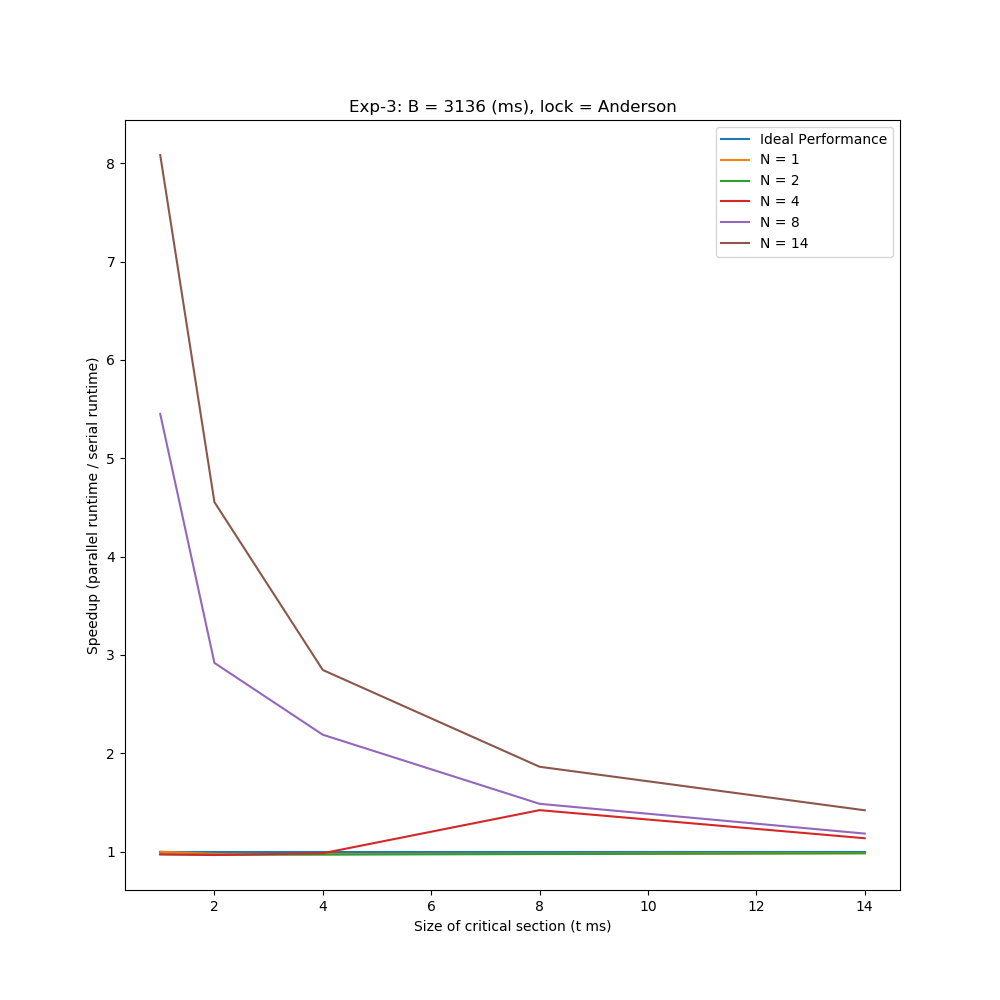
\includegraphics[scale=0.5]{graphs/exp3_a.png}\\
%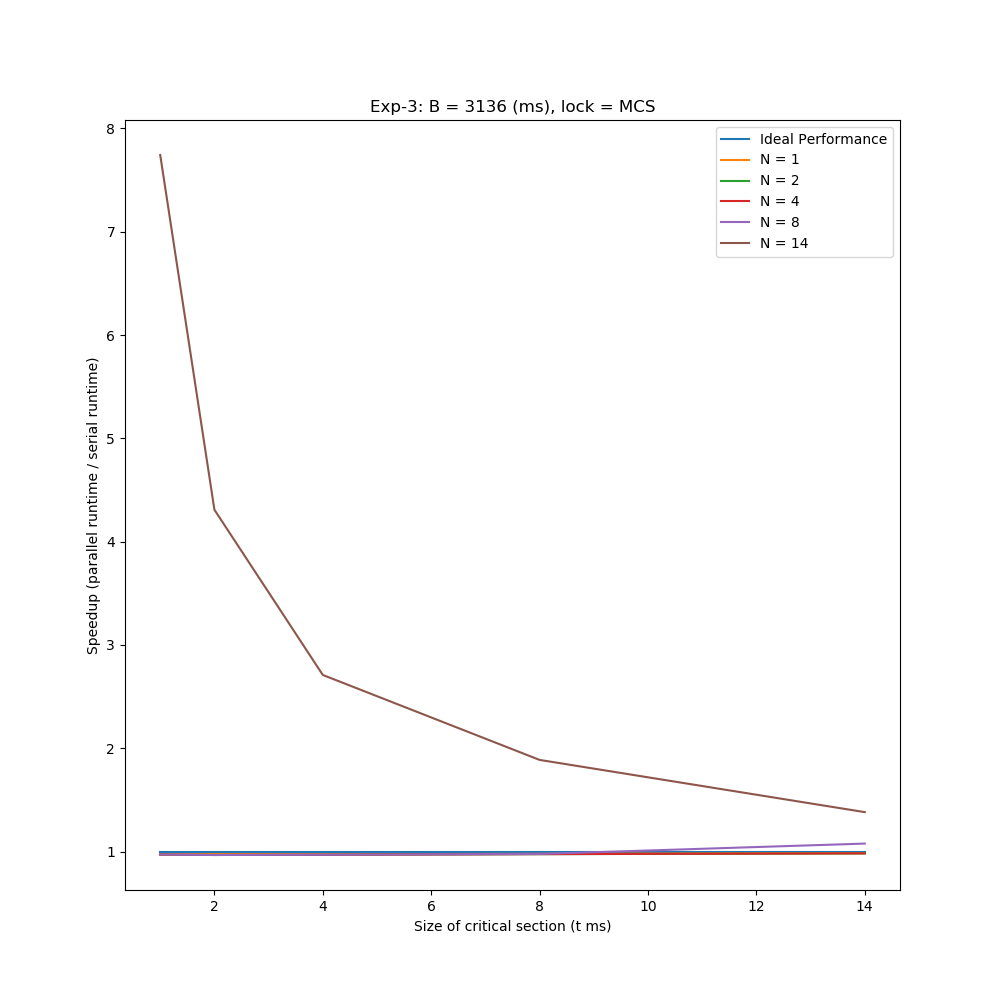
\includegraphics[scale=0.5]{graphs/exp3_m.png}\\%

\section{Analysis}

\subsection{Experiment 1: Idle Lock Overhead}

\subsection{Experiment 2: Lock Scaling}

\subsection{Experiment 3: My Test}

\end{document}
